\documentclass{article}

\usepackage{simcmag}
\usepackage[export]{adjustbox}

\date{\hspace{30mm}}
\currentvolume{1}

\newcommand{\simcmagcredits}{
  \footnotesize
  \begin{tcolorbox}[boxrule=1.0pt,colback=white,hbox,before upper*=\begin{tabular}{l},after upper*=\end{tabular}, sharp corners,left=-5pt,right=-5pt]
  Editor-in-Chief: Edward Y. \\
  Staff Writers:\\
  \begin{tabular}{ll}
    Cecilia S. & Edward Y. \\
    Joyce H. & Michael Y.\\
    Owen X. & Rohan D. \\
    William Y. F. & William G. 
  \end{tabular}\\
  Guest Writers: \\
  \begin{tabular}{ll}
    Samarth D. & \hspace{1.8mm} Jason Y.
  \end{tabular}
  \end{tcolorbox}
}

% uasage of picinpar:
%\begin{window}[1,l,\includegraphics{},caption]xxxxx\end{window}

% usage of window:
% \begin{window}[2,r,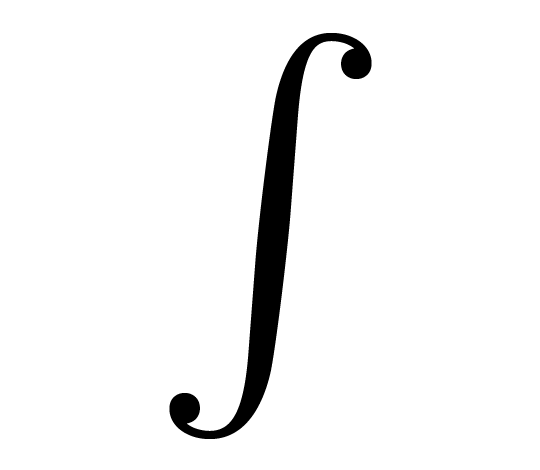
\includegraphics[width=1.0in]{img/logo.png},\centerline{a picture}]
% Duis aute irure dolor in reprehenderit in voluptate velit esse cillum dolore eu fugiat nulla pariatur. Excepteur sint occaecat cupidatat non proident, sunt in culpa qui officia deserunt mollit anim id est laborum
% \end{window}

%%%%%%%%%  Front matter   %%%%%%%%%
\begin{document}
\maketitle
\begin{minipage}[t]{.45\textwidth}\thispagestyle{empty}
  \vspace{-11mm}
  \tableofcontents
\end{minipage}% 
\begin{minipage}[t]{.1\textwidth}\thispagestyle{empty}
  \;
\end{minipage}% 
\begin{minipage}[t]{.45\textwidth}\thispagestyle{empty}
  \setlength{\parskip}{5pt}
  \vspace{-7mm}
  {\itshape
  Dear Reader:

  Welcome to the inaugural issue of \emph{The Circle}, a math literacy magazine founded by the student leaders of the Seattle Infinity Math Circle.

  Our mission is to advocate for the world of math, to provide a window into its fascinating history, its distinctive culture, and its many untold stories.

  We hope to break the negative stereotype towards math students and, most importantly, we'd love this to be a voice for you, our dearest mathematical friends.

  We're excited to start this journey with you and plan to fill each issue with our favorite math gems, biographies, fun facts, and much more!
  
  Have fun reading!

  Sincerely,\\
  Edward Yu\\
  Editor-In-Chief
  }
\end{minipage}

\vspace{3mm}

\closearticle

\begin{multicols}{3}{

\articletitle{Goldbach's Conjecture}{Joyce Huang}{}

\begin{center}
    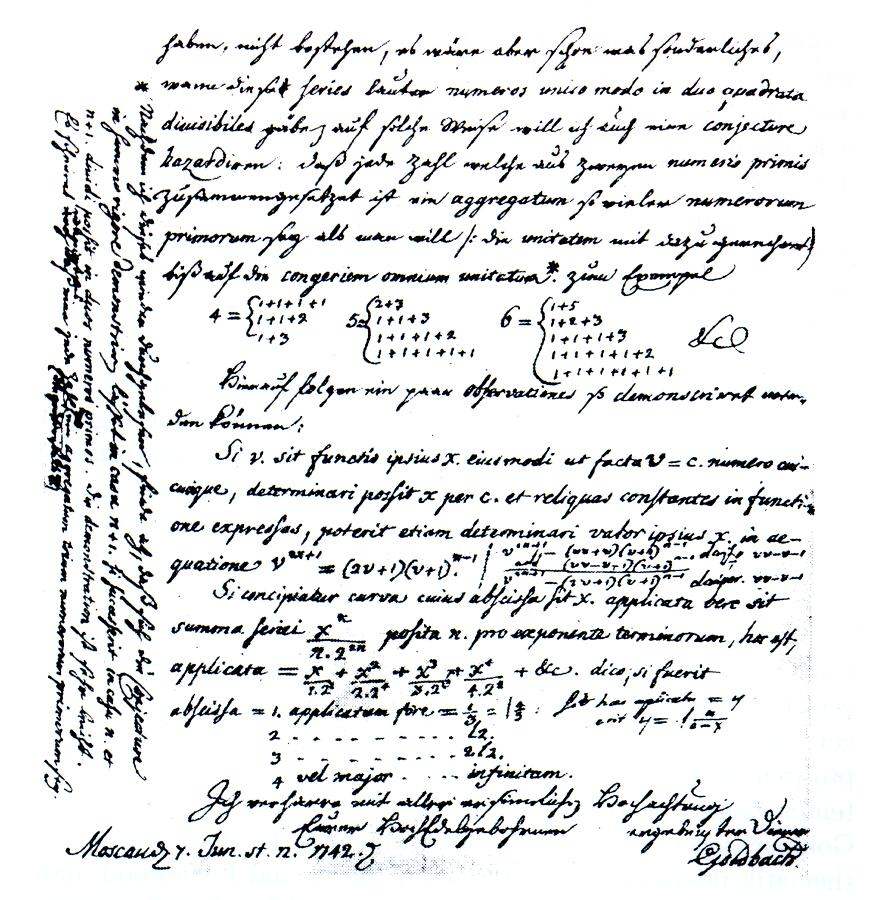
\includegraphics[scale=0.18]{Magazines/img/Vol1/goldbach-conjecture.jpg}
\end{center}

Goldbach’s Conjecture is one of the most famous unsolved math problems in the world. It states that every even integer greater than two can be expressed as the sum of two primes. 

The conjecture is named after Christian Goldbach, a German mathematician who proposed it in 1742. On June 7th of that year, he wrote a letter to Leonhard Euler, another famous mathematician, that contained a conjecture he found: ``If an integer $n$ can be expressed as the sum of two primes, then it can also be expressed as the sum of $k$ primes, where $k$ is an integer from 2 to $n$.'' He also wrote a second conjecture in the margin of the letter: ``Every integer greater than 2 can be expressed as the sum of three primes.'' 

In Euler’s response letter, he recalled a previous conversation between the two, where Goldbach said that both of the above conjectures were results of another conjecture, ``Every even integer greater than 2 can be expressed as the sum of two primes,'' which is the final, strongest version of the conjecture.  

Even almost three hundred years after Goldbach first proposed his conjecture, it is still an open problem. Most mathematicians believe it to be true, and as of 2013, computers have confirmed it for numbers up to over $4\cdot10^{18}$ (4,000,000,000,000,000,000). 

One way some mathematicians have approached proving this conjecture is through the probabilistic method. The general idea is that as the even integer grows larger, there are more and more ways to express it as the sum of two integers, so the likelihood of there being at least one pair of two primes increases. While probability does not provide a rigorous proof, it has given strong evidence that large even numbers are the sum of not just one, but many pairs of primes.

In their exploration of this conjecture, mathematicians became interested in Goldbach’s function. Goldbach’s function outputs the number of ways to express an even integer as the sum of two primes. Its graph is pictured below:
\begin{center}
    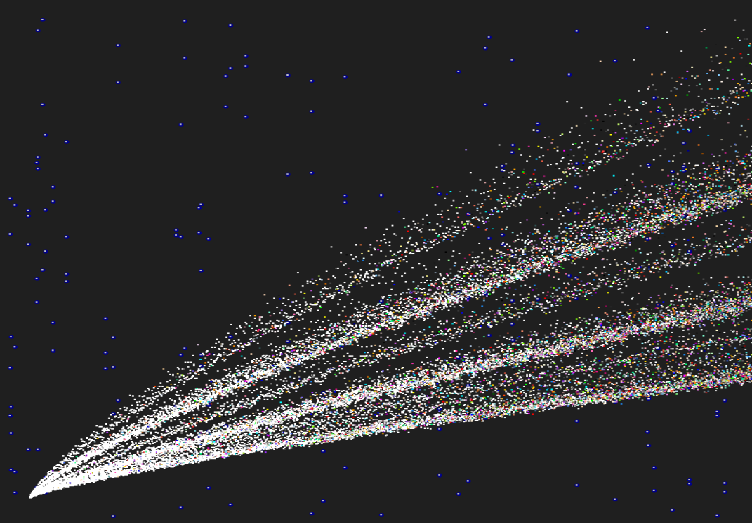
\includegraphics[scale=0.4]{Magazines/img/Vol1/goldbach-comet.png}
\end{center}
Mathematicians call the graph Goldbach’s Comet because the shape represents a comet and its tail. The streaks in the graph show that there are different groups of even integers whose number of ways to be expressed as the sum of two primes increase at different rates. The streaks are based off of the odd prime factors of the input. For example, the lowest streak consists of numbers who are either powers of 2 or can be expressed as $2p$, where $p$ is a prime number. Inputs of powers of 2 correspond to the lowest outputs because they are not divisible by any odd primes, which means if two odd numbers $a$, $b$ sum to the power of 2, they are never both divisible by any odd prime. Thus, the “ruling out” of pairs of odd numbers never overlaps, resulting in a smaller output. Furthermore, the groups appear to increase linearly.

Despite all the evidence suggesting that Goldbach’s conjecture is true, it is important to remember that it has not yet been proven, and we won’t know for sure until someone proves it. That someone could be anyone. It could even be you!
\begin{center}
    
\includegraphics[scale=0.3]{Magazines/img/Vol1/stick_figure1.png}
\end{center}
\closearticle
\clearcolumn
\articletitle{The Golden Ratio}{William Gvozdjak}{}

\epigraph{
  The golden ratio, also known as the divine proportion, golden mean, or golden section...
}{\href{https://mathworld.wolfram.com/GoldenRatio.html}{``Golden Ratio'' (\emph{MathWorld})}}
The golden ratio is given a majestic name in math. It’s frequently known to be somehow “pleasing” to humans and is represented by the Greek letter $\phi$ (pronounced phi). But one thing is still not clear to many people: what really is the golden ratio, and why on earth is it so “important”? 

Let’s first start with how the golden ratio is defined. At its most basic form, it’s the irrational number $\phi = \frac{1+\sqrt5}2$, the positive solution to the quadratic equation $x^2-x-1=0$. It is also frequently defined as $\frac ab$, where $\frac{a+b}a = \frac ab$ (which has a nice graphical interpretation in the following diagram):

\begin{center}
    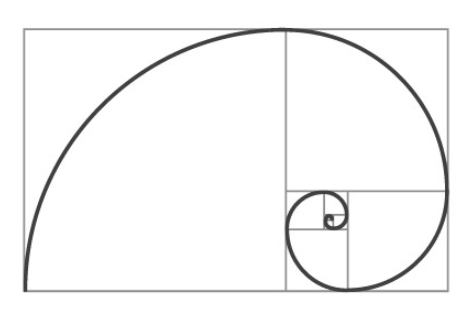
\includegraphics[scale=0.35]{Magazines/img/Vol1/golden-ratio.png}
\end{center}

None of these representations, however, really give any reason as to why the golden ratio is so interesting. Here’s an example that starts to be more interesting.

The Fibonacci Sequence, where the $n$th term is denoted as $F_n$, is a sequence of numbers where each number is the sum of the two numbers before it. Mathematicians frequently start the sequence by defining $F_0=0$ and $F_1=1$, and the sequence therefore continues with $1$, $2$, $3$, $5$, $8$, $13$, etc. A natural question is then: is there some closed-form formula for the $n$th term of the sequence?

The answer is Binet’s Formula. Binet’s Formula, out of nowhere, has a fascinating connection to the golden ratio: the $n$th term of the Fibonacci Sequence, $F_n$, is $\frac{\phi^n - \psi^n}{\sqrt5}$, where $\phi$ is the golden ratio and $\psi$ the conjugate of the golden ratio, $\frac{1-\sqrt{5}}{2}$. The Fibonacci Numbers, which is a sequence of integers, not only has a closed-form formula with irrationals, but the golden ratio, out of all numbers!

Another natural question that follows the definition of the Fibonacci Numbers is: how do the numbers behave as the sequence progresses further and further? One way we can quantify this is to find how the ratio between consecutive Fibonacci Numbers changes along the sequence. This is written as $\lim_{n\to\infty}\frac{F_{n+1}}{F_n}$ (read as ``the limit of $\frac{F_{n+1}}{F_n}$ as $n$ approaches infinity''). As the index of the Fibonacci Numbers increases, what number does the ratio between consecutive Fibonacci Numbers approach?
To compute this, we can use a neat trick: we know that $\lim_{n\to\infty}\frac{F_{n+1}}{F_n}=\lim_{n\to\infty}\frac{F_n}{F_{n-1}}$. We can therefore write an equation to find that quantity using the definition of the Fibonacci Numbers: $F_{n+1}=F_n+F_{n-1}$. Letting $x=\lim_{n\to\infty}\frac{F_{n+1}}{F_n}$, we have:

{\footnotesize\begin{align*}
    F_{n+1}&=F_n+F_{n-1}\\
    \frac{F_{n+1}}{F_n}&=\frac{F_n}{F_n}+\frac{F_{n-1}}{F_n}\\
    \frac{F_{n+1}}{F_n}&=1+\frac{1}{\frac{F_n}{F_{n-1}}}\\
    \lim_{n\rightarrow\infty} \frac{F_{n+1}}{F_n}&=1+\frac{1}{\lim_{n\rightarrow\infty} \frac{F_{n}}{F_{n-1}}}\\
    x&=1+\frac{1}{x}\\
    x^2&-x-1=0.
\end{align*}}


But this is exactly one of the definitions of the golden ratio: a solution to the quadratic equation $x^2-x-1=0$ (the second solution is negative, which clearly cannot be the ratio of two positive Fibonacci Numbers)! This means that the ratio of two consecutive Fibonacci Numbers tends to the golden ratio as the sequence progresses, yet another surprising connection between the Fibonacci Numbers and the golden ratio.

However, the golden ratio isn’t just interesting in algebra. It also comes up in surprising situations in geometry, as well. Let’s look at an example problem.

Suppose that we have a regular decagon: a polygon with $10$ sides that all have equal length. Now, let’s take its circumcircle: draw a circle going through all 10 vertices of the polygon. What is the ratio between the radius of the circumcircle of the decagon and the length of a side of the decagon?

\begin{center}
    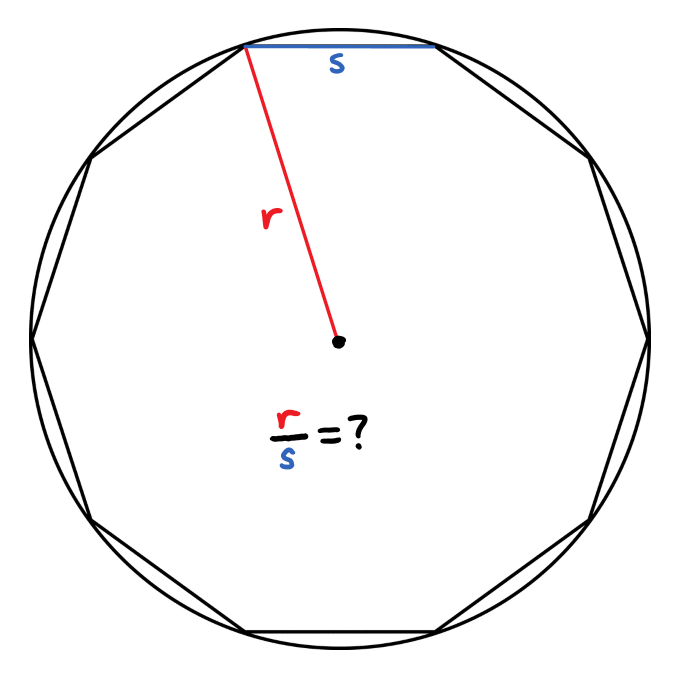
\includegraphics[scale=0.25]{Magazines/img/Vol1/golden-ratio3.png}
\end{center}

Let’s suppose that the center of the circumcircle is the point $O$. Then, note that we can create a right triangle by dropping an altitude from $O$ to the midpoint of the side. We then have a right triangle with hypotenuse $r$ and leg $\frac s2$.

\begin{center}
   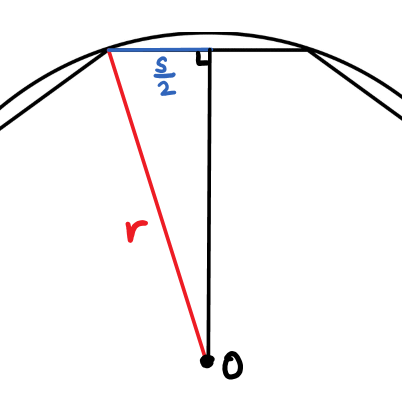
\includegraphics[scale=0.35]{Magazines/img/Vol1/golden-ratio4.png}
\end{center}

If we find the ratio between $r$ and $\frac{s}{2}$, we know the ratio between $r$ and $s$. To find $\frac{r}{s/2}$, notice that it is equal to the reciprocal of the $\sin$ of the angle at $O$, as $\sin$ is opposite over hypotenuse! Therefore, we must simply find how large the angle at $O$ is.

We can find the angle at $O$ by cleverly using symmetry: notice that the angle we want is just $\frac1{20}$ of the entire circle, which is $18^\circ$.

\begin{center}
    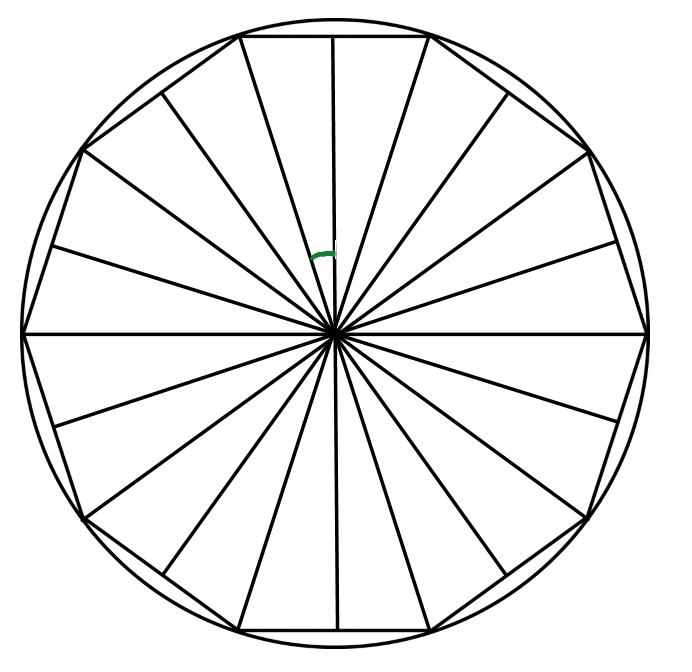
\includegraphics[scale=0.25]{Magazines/img/Vol1/golden-ratio5.png}
\end{center}

Therefore, we know that $\frac{r}{s/2} = \frac1{\sin 18^\circ}$, so $\frac rs = \frac1{2\sin 18^\circ}$. What is the value of $\sin 18^\circ$? There are various ways to calculate this\footnote{You can read about them \href{https://math.stackexchange.com/questions/2140356/various-methods-to-find-value-of-sin-18-circ}{here}.}, but once we do, we find that $\sin 18^\circ = \frac{\sqrt5-1}4$. Therefore, we know that $\frac rs = \frac1{2\frac{\sqrt5-1}4} = \frac{\sqrt5+1}2$, exactly the golden ratio!

In sum, the golden ratio is fascinating in mathematics simply due to its ubiquity: why is such an arbitrary number so universally found and used? So, the next time the number $\frac{1+\sqrt5}2$ shows up in a problem, take a brief pause to appreciate the strange appearance of the golden ratio.
\closearticle


\articletitle{Minesweeper is Hard}{William Y. Feng}{}

My friend keeps sending me half-finished minesweeper grids and challenging me to solve them:
\begin{center}
    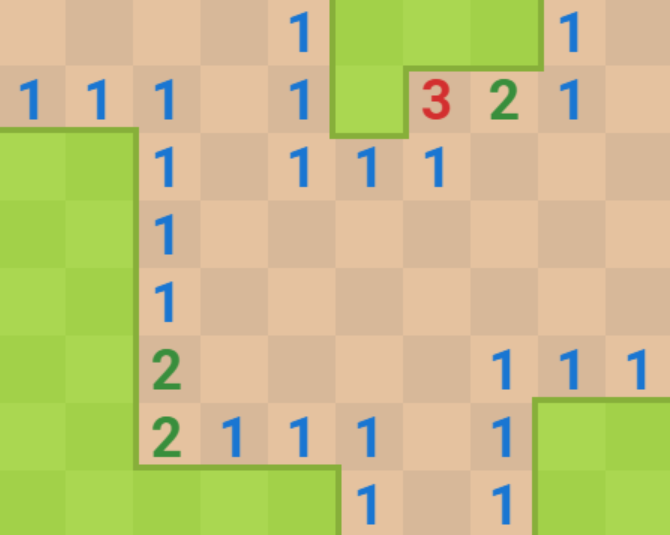
\includegraphics[width=2in]{Magazines/img/Vol1/Minesweeper_fig1.png}
    
    \small{A half-finished Minesweeper grid}
\end{center}

The thing is, my friend likes to mess with me sometimes, so I’m not convinced that it’s even possible to place mines on the grid in a way that’s consistent with the numbers. I want a fast way to check that any grid my friend sends me is solvable---specifically, I want a computer program that takes an $n \times n$ grid representing a partially-complete minesweeper grid as input and outputs whether there exists a configuration of mines consistent with the numbering. This problem is called MINESWEEPER. It’s important to note that the program doesn’t have to tell me what, if any, placement of mines makes the numbers consistent, simply a  “YES” or “NO.” (If my friend isn’t trolling me, then the task of finding a placement of mines can be left up to me.)

I also want the number of operations the program does to be bounded by some polynomial in $n$. This is a really loose bound, but it’s a nontrivial one---imagine a program that simply enumerates all possible ways to assign mines to the unrevealed squares and checks whether any assignment works. This could take up to the order of $2^{n^2} \cdot n^2$ operations, which is definitely not a polynomial in $n$. Such a program is said to run in polynomial time or to be a poly-time algorithm.

\subheader{CIRCUIT-SAT}

I might not have a program that can solve this problem in polynomial time, but I do have a magic box that takes in any arbitrary logic circuit as input and instantly determines whether there exists some combination of input bits that results in the output bit being 1. This problem is called circuit satisfiability, or CIRCUIT-SAT for short. For instance, if I put this circuit into the magic box:

\begin{center}
    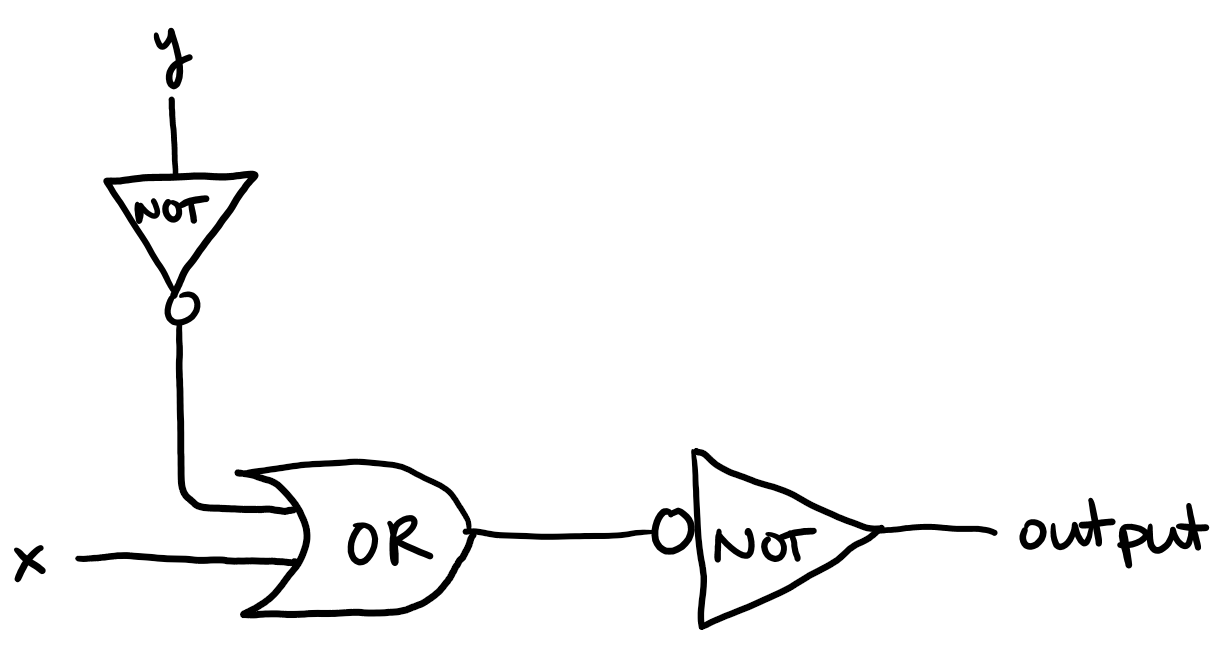
\includegraphics[width=2in]{Magazines/img/Vol1/Minesweeper_fig2.png}
    
    \small{Sample logic gate}
\end{center}

Then it will tell me, in a single operation, that the answer is YES. If we set $x=0$ and $y=1$, then the output will be 1 as well. The box won’t tell me what combinations of inputs will output a 1, it just tells me YES or NO. Using this magic box, I’m able to easily determine if one of my friend’s minesweeper grids is solvable. Here’s what my proposed program does:
\begin{enumerate}
\item Receives as input an $n \times n$ minesweeper grid
\item Write a sub-program in C where:
    \begin{enumerate}
    \item The input consists of proposed locations for mines in the grid
    \item The output is a binary representing whether the input is consistent with the grid
    \end{enumerate}
\item Compile this C code to a circuit using a C to HDL tool
\begin{enumerate}
    \item The compiled circuit takes in proposed locations for mines encoded in binary and outputs whether the input is consistent with the original grid
\end{enumerate}
\item Plug this circuit into my magic box and output its result
\end{enumerate}

You’ll have to trust me that the circuit resulting from step 3 has a polynomial number of gates in terms of $n$, but intuitively, since we’re only looping through every cell in the grid once and doing 8 checks per grid, the circuit should be relatively small.


\subheader{Going the other way}

To get revenge on my friend, I send them a large logic circuit with several inputs and one output, and challenge them to determine whether there exists some combination of input bits such that the output bit is a 1. Here’s the circuit I sent them:

Unlike me, they don’t have a magic box that can immediately tell them the answer. But, unlike me, they’re actually good at minesweeper and can instantly tell whether a partially-filled minesweeper grid has a solution just by looking at it. So here’s what they did:

\begin{center}
    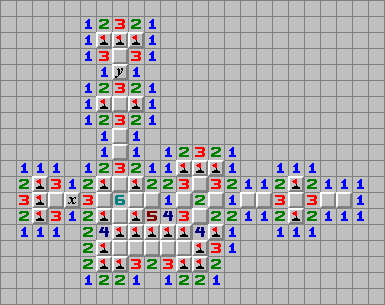
\includegraphics[width=2in]{Magazines/img/Vol1/Minesweeper_fig3.png}
    
    {\small When life gives you logic circuits, turn them into \href{http://www.formauri.es/personal/pgimeno/compurec/Minesweeper.php}{minesweeper grids}}
\end{center}

Dark grey cells are assumed to be 0, and flagged cells must logically have mines in them. The rightmost flag corresponds to the output wire, the square labeled $x$ on the left side of the grid corresponds to input wire $x$, and the square labeled $y$ near the top corresponds to input wire $y$. Reasoning out the grid, we can determine that the output square has a mine if and only if the logical statement “not ($x$ or not $y$)” is true, which corresponds exactly with the logical circuit I gave my friend.

In fact, my friend is able to convert any logic circuit into a minesweeper grid using some simple “widgets” representing wires and all the different kinds of gates. Furthermore, it only requires a grid size that’s polynomial in the number of gates in the circuit. This, together with their superhuman minesweeper-solving skills, allows them to solve any logic circuit I present to them in polynomial time.


\subheader{Closing remarks}

This was a brief introduction to complexity theory, and in this article we showed (non-rigorously) that the two problems MINESWEEPER and CIRCUIT-SAT (short for circuit satisfiability) can be used to solve one another. There are a lot of unsolved problems in this field, such as the famous P=NP conjecture, and if this article was interesting, I recommend looking into it further with the resources.
}
\closearticle


\articletitle{Galois Biography}{Michael Yang}{}

\epigraph{Science is the work of the human mind, which is destined rather to study than to know, to seek the truth rather than to find it.}{\'Evariste Galois}

\begin{center}
    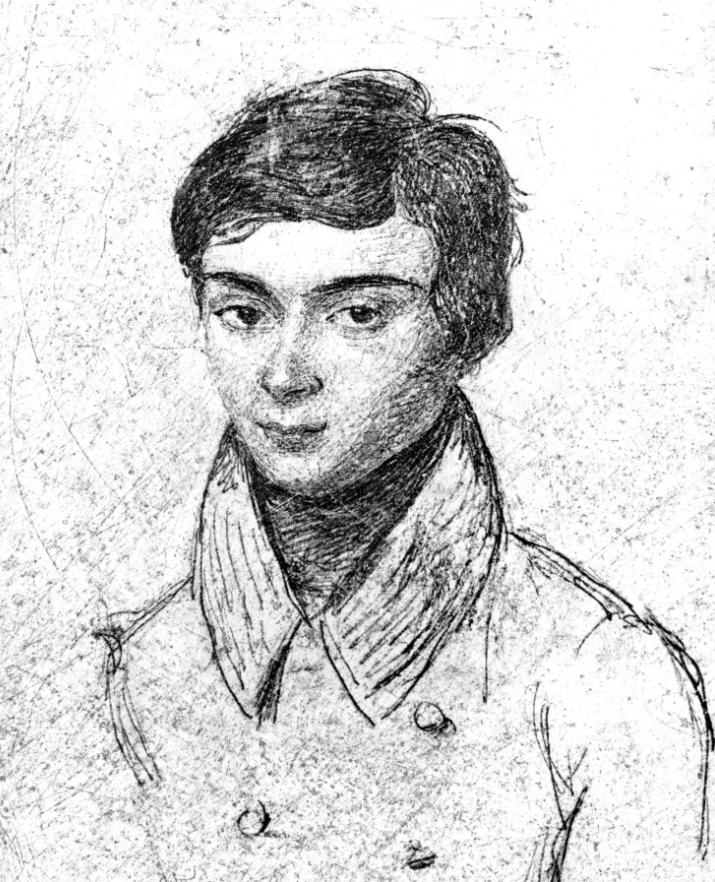
\includegraphics[scale=0.45]{Magazines/img/Vol1/galois.png}
\end{center}

Évariste Galois was a French mathematician who lived in the early 1800s. Born on October 25th, 1811 in the village of Bourg-la-Reine, France, Galois’ interest in mathematics started when he was young. He started to seriously study the subject at the age of fourteen when he read the works of contemporary mathematicians such as Legendre; famously precocious, it is said that he understood many of these works completely after the first reading. 

Galois is often credited as being the founder of the modern branch of mathematics known as abstract algebra. This began with him formalizing the definition of a mathematical structure known as a group, which other people had thought of but had never rigorized. From this, Galois laid down some of the fundamental framework of what is now called group theory, which (loosely speaking) is the study of symmetry and the ways in which something can be symmetrical. He also was the first to focus on a field of math aptly named Galois Theory, which is an extension of group theory into other areas of study. Together, these two fields are surprisingly versatile, being used in everything from counting the number of symmetries of a Rubik’s cube to being able to determine whether a given polynomial equation has roots that can be expressed with radicals.

\begin{center}
    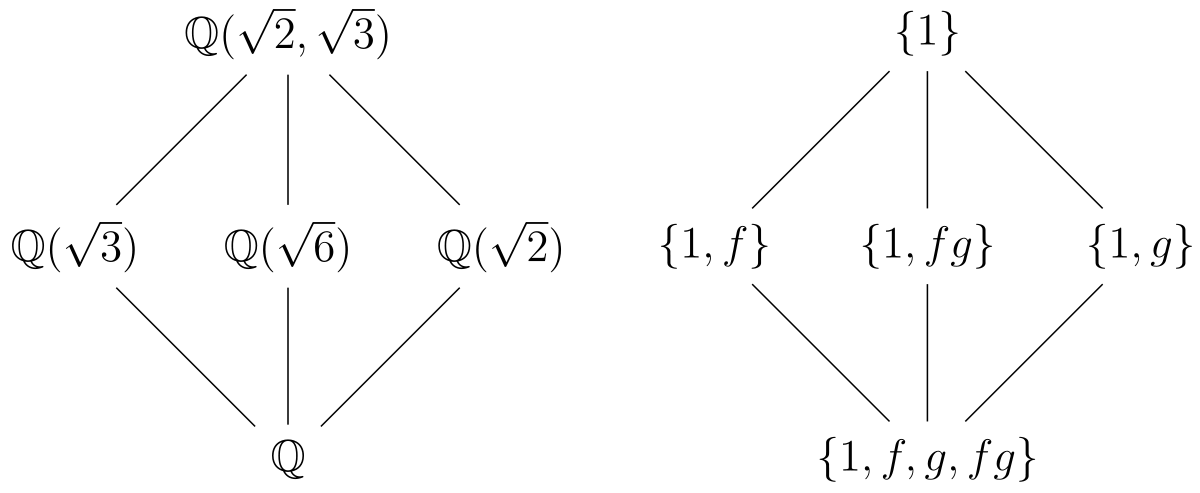
\includegraphics[scale=0.12]{Magazines/img/Vol1/galois-theory.png}
\end{center}

Galois might be as well-known for the volatility of his persona as for the genius of his mathematical works. Growing up in a France rocked by political instability, Galois became heavily involved in the Second French Revolution. After making a threatening speech against the king, he was arrested, and then was arrested again shortly after for illegally wearing a uniform. Galois’ time spent in mathematics was also interlaced in this political fervor; at around the same time, Galois was expelled from the French institute École Normale because he attacked the director in a letter to the newspaper. 

Near the end of his life, Galois spent much of his time consolidating all of his mathematical findings into one long letter. Despite it being written very hastily, it touched upon incredibly deep results; some of the theorems he included weren’t proved until more than a century later! 

Shortly after the completion of this letter, Évariste Galois died on May 30th, 1832, in a duel that was likely sparked by political unrest. He was only twenty years old. But despite his unfortunately short life, Galois still is regarded as one of the most important mathematicians of the modern era. Unlike some of his contemporaries, the collection of all his published writing barely spans sixty pages; what they contain, though, is the genesis of some of the fields that are most essential to mathematical research today. And while Galois might ultimately be remembered as perhaps one of the more mysterious figures in math, there is no question that he played an essential role towards getting the subject where it is today. 
\closearticle


\articletitle{An Overlooked, but Massive Strategy}{Rohan Dhillon}{Mass Points are Quite the Balancing Act}


As I walked out of the AMC 8 testing room in 2019, I had only one question: how the hell do you do problem 24? (My mind, preferring algebra, did not want to go hunting for similar triangles in a geometry problem during a 40 minute test.) 

\vspace{5mm}
\noindent\fbox{\begin{minipage}{0.28\textwidth}
{\footnotesize In triangle $ABC$, point $D$ divides side $\overline{AC}$ so that $AD:DC=1:2$. Let $E$ be the midpoint of $\overline{BD}$ and let $F$ be the point of intersection of line $BC$ and line $AE$. Given that the area of $\triangle ABC$ is $360$, what is the area of $\triangle EBF$?}
\begin{center}
    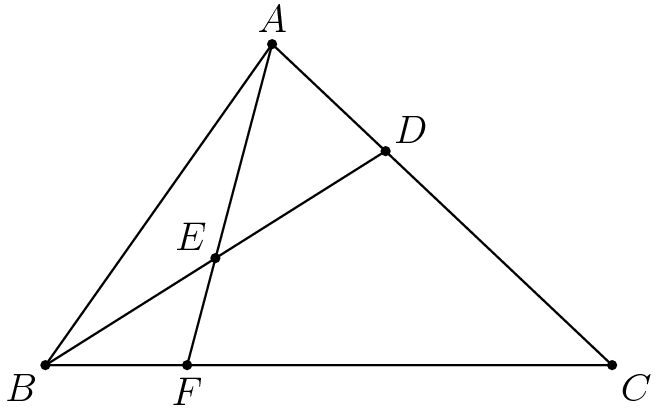
\includegraphics[scale=0.20]{Magazines/img/Vol1/mass_point_2019_AMC8_P24.png}
\end{center}
\end{minipage}}
\vspace{5mm}

At first, the problem seemed innocuous: simple at best, a little bashy at worst. However, as I began frantically scribbling notes, the problem manifested itself as almost impossible. Coming out of the room, my annoyance was immeasurable; I quickly headed over to a consortium of the so-called “mathy” people of my school, three of whom got the answer: one by guessing, and the other two by drawing a very accurate diagram. But, still to all of us, the true method had yet to reveal itself.



During my next math class, our math teacher taught us a clever, and yet rarely taught, way to solve certain geometry problems that I want to share with you now; this method is called mass points, best taught through the example of that AMC 8 problem (admittedly, you could also solve it using triangle ratios, but mass points will annihilate the problem in under a minute). 
Below, in the problem statement, we have two crucial elements signifying that the method mass points might be viable: information about ratios and line intersections. Before we begin solving this problem, it’s important to note that the crux of mass points comes from physics: specifically, if you have two masses on a balance beam, they have to satisfy a special relationship for the beam to be balanced: taking either mass and multiplying it by the distance from that mass to the fulcrum (the “balance point” of the beam) gives you the same quantity. 

We can employ this property by using lines in the diagram as beams. For example, take $AC$: we know that $AD$ and $DC$ are in a 1 to 2 ratio, so we can assign $A$ and $C$ masses that make $AC$ a ``balanced beam'' (one of the great things about math as opposed to physics: you can just assign things). Theoretically, we could give them any mass, but, for simplicity’s sake, let’s just say that the mass of $A$ is 2 and the mass of $C$ is 1 (we can verify that this satisfies the “balancing act” we’re trying to fulfill: $A$ times $AD$ equals $C$ times $CD$). Great. Now what?

Another great property we can exploit in math (do not try this in your physics class) is to set the mass of $D$ to the mass of $A$ plus the mass of $C$, thereby setting it to 3. But, of course, this begs the question: why? Well, we want the entire diagram to be balanced and so we wish the line segment containing $D$ to be balanced, but this line segment will have $AC$ on one side and thus it has to balance all of $AC$, which is why we set D to the “total mass” of the line segment. And now the optimal strategy is to spam mass points until we’ve gotten the mass of every point we can, and hopefully we can find some ratio information that’s useful to us. 
In this problem, that approach looks something like this: we have that $D$ has mass 3 and the $E$ is the midpoint of $BD$; therefore, $B$ must have mass 3, and $E$ must have mass 6. Since we know that $A$ has mass 2, we can deduce that $F$ must have mass $6 - 2 = 4$ (you could confirm this by looking at $BC$ or $AF$). 

\begin{center}
    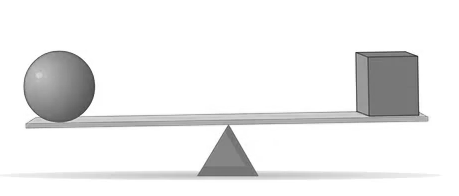
\includegraphics[scale=0.40]{Magazines/img/Vol1/mass-point.png}
\end{center}

Just from those simple calculations, we’ve deduced that $BF : FC = 1 : 3$, and $EF : EA = 1 : 2$. Thus $BF : BC = 1 : 4$ while $EF : AF  = 1 : 3$. This tells us that EBF's base is 4 times smaller than ABC’s and that its height is 3 times smaller (this is because their heights are in the same ratio as EF and AF). Therefore, the area of EBF must be $4 \cdot 3 = 12$ times smaller than ABC, so our answer is 30. 


While this problem may be simpler than most you will probably encounter in the future, I hope that it served as a good introduction to mass points–particularly, their simplification of laborious triangle-hunting (I think that’s a term). Before you go, I just want to remind you of when to use mass points. If you have ratio information and intersections, or you’re simply hunting for similar triangles on an easier problem, by all means use it; however, it’s unlikely that simple mass points will be enough for the likes of harder AMC 12 problems or beyond, so always try multiple methods, perhaps in conjunction. 
Mathematics is a field constructed out of basic elements that is rich in information and ripe for discovery, if only we are willing to tilt our heads in the right way--and that’s it for the math (and puns) from me!
% \begin{center}
%     
\includegraphics[scale=0.28]{Magazines/img/Vol1/stick_figure2.png}
% \end{center}
\closearticle

\articletitle{Axiom of Choice}{Cecilia Sun}{}

During the early twentieth century, the world of mathematics was roused in heated debate and controversy as mathematicians attempted to systemize and rigorize mathematics. Their goal was to construct the foundations under which past and future mathematics could be built onto. Yet, as it turns out, when we play around with the fundamental rules of our mathematical universe, we are bound to run into results that contradict our intuitive understanding of the ways in which mathematics should work. Perhaps the most famous of these controversies was the Axiom of Choice, which, when it was first conceptualized, is said to have broken mathematics. 

The modern formulation of the Axiom of Choice is as follows:

Let $(A_i)_{i\in I}$ be a collection of nonempty sets. There is a \textit{choice function} $f:A_i\to \bigcup_{i\in I}A_i$ such that for every $i\in I$, $f(A_i)$ is an element of $A_i$.

\begin{center}
    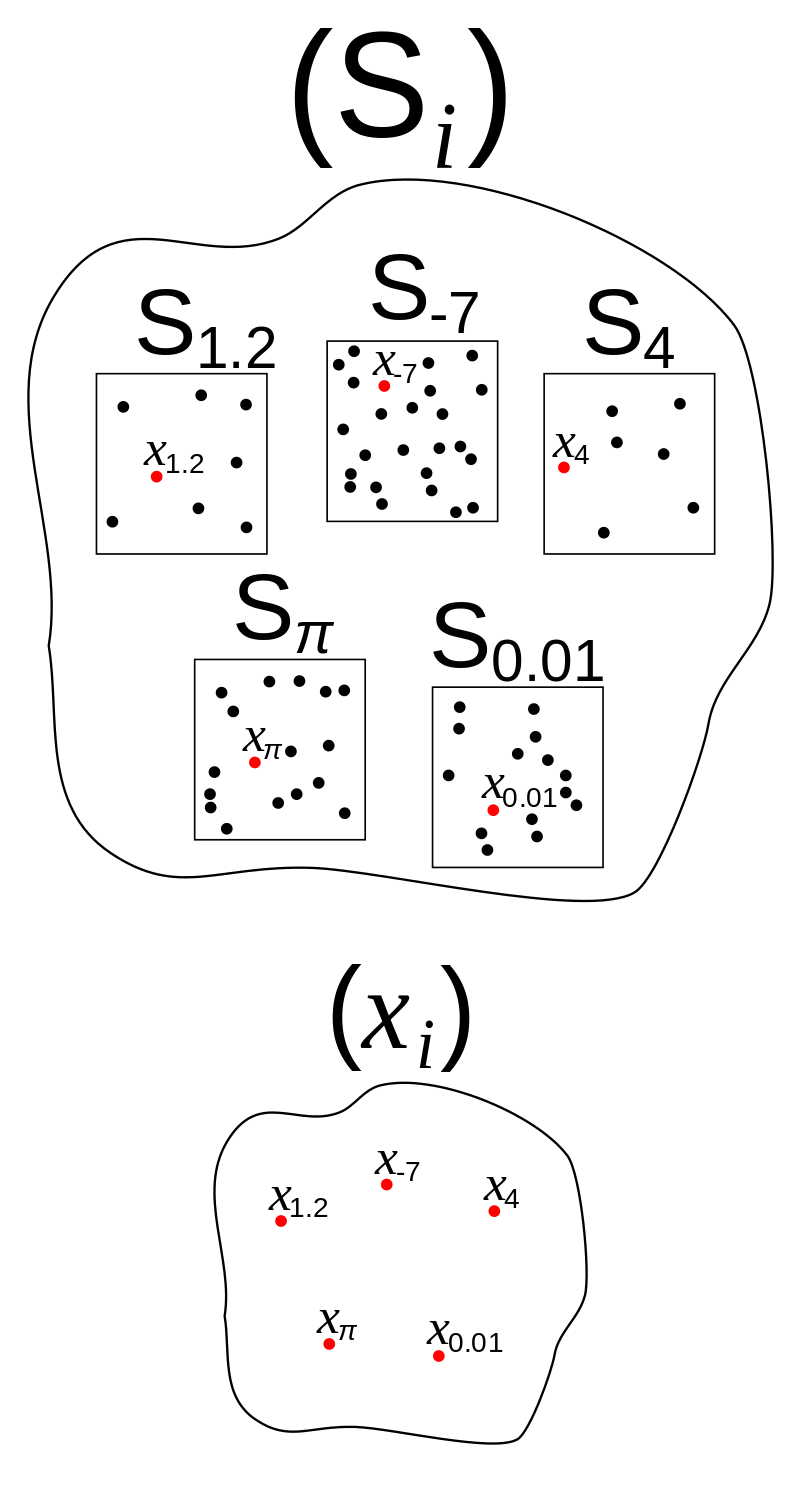
\includegraphics[scale=0.18]{Magazines/img/Vol1/axiom_of_choice.wikipedia.png}
\end{center}

This is a formal way of saying that there is a function that, given a bunch of sets, we can choose exactly one element from each of the sets. To understand why this seemingly innocuous axiom caused such uproar in the mathematical community, we will need to understand why it was discussed in the first place, which will require us to discuss the Well-Ordering Principle. 

We define a well order on a set to be a relation $\preceq$ that satisfies the following properties:
Irreflexivity: If a$\preceq$ b and b$\preceq$ a, then a=b.
Transitivity: If a$\preceq$b and b$\preceq$ c, then a$\preceq$ c.
Totality: Given any two elements a, b $\in$ A, either a$\preceq$ b or b$\preceq$ a.
Well-ordered: Any nonempty subset S$\subseteq$ A has a $\preceq$-minimal element.

The first three conditions define a total order – intuitively, this can be thought of as any “ordering” of things. For instance, the “less than” relation on the real numbers, or the alphabetization of strings of letters are all examples of total orders. 

The last condition makes a relation a well order – essentially, it tells us that in any subset of the set we defined our relation on, we can find an element that is “minimal”, or one that is “less than” all of the others.

However, it’s hard to find well orders on a lot of common sets! For instance, there is no least element of the open interval of reals between $0$ and $1$. 

The Well-Ordering Principle states that every set has a well order. In other words, given any set, we can always find an ordering such that every subset has a least element – even the reals! As such, mathematicians were highly skeptical of the Well-Ordering Principle when it was first formulated, even going as far to state that it was “obviously false”.

On the other hand, mathematicians had already been using the Axiom of Choice freely in their proofs. So, when, in 1904, Zermelo proved that the Axiom of Choice and the Well Ordering Principle imply each other, meaning that they were either both true or both false, the math community erupted in scandal and outrage. 

It turns out that both the Axiom of Choice and its negation both imply statements that should intuitively be true. For instance, believing in the Axiom of Choice implies that every set has a cardinality (in other words, a size), and that the countable union of countable sets is countable. However, believing in its negation implies that sets have a well-defined notion of volume, and that there is an infinite set of reals that does not contain a countably infinite set. 

Though the Axiom of Choice was initially controversial, it is nowadays accepted as an axiom by most mathematicians and is included in the standard form of axiomatic set theory, Zermelo-Fraenkel set theory with the Axiom of Choice (ZFC).
\closearticle

\articletitle{A Game of Pinching Pennies}{Edward Yu}{}

\epigraph{Life is like a puzzle. The more you try to resolve it, the more you will get trapped in the mystery.\dots}{Rahul Singh}

That is exactly how I felt after seeing the “weekend puzzle” sent to my school’s math team one Friday afternoon in January. Our longtime math coach, Mr. Dean Ballard, had introduced the puzzle a few weeks ago not only to us math team members, but also to the whole world via the Riddler, a column of the prestigious news analysis website FiveThirtyEight. First published in ``ye olden days'' back in 1907, it is a simple game with rules that anyone can understand:

Alex has some number of pennies, which Bill divides into two piles. They take turns, with Alex going first. Each turn, a player either removes any number of pennies from one pile, or an equal number of pennies from both piles. Taking nothing is not allowed.

\begin{center}
     
\includegraphics[scale=0.8]{Magazines/img/Vol1/play_game.png}
\end{center}

The winner will be the one who takes the last penny. Since, of course, Alex and Bill are both geniuses, they will play perfectly to optimize their chances of winning. What numbers of pennies can Alex choose at the beginning to guarantee a win?


In fact, Mr. Ballard says this game was once a bonus problem for his sixth-grade math class. I (and some friends), veteran high-school math enthusiasts, will certainly have no problem solving this… right? As it turns out, I was stumped by this problem for several days, and almost anyone would be challenged to solve it. One student who struggled with the game described: “There must be a pattern – I know it. I just can’t see it.” This sums up the agony of working on such a seemingly easy problem.


Mr. Ballard was not trying to train the Math Team to become future gamblers, nor was he trying to make con artists out of us. Instead, as a passionate puzzle-lover, he is bringing us to see the connections between an obscure game and a well-known pattern.
As for the real answer to the puzzle, it is surprisingly related to the famous Fibonacci numbers: 1, 1, 2, 3, 5, 8, 13…, where each number is the sum of the previous two—and has a much deeper relation to the golden ratio, $\phi = \frac{1+\sqrt{5}}2$.
\begin{center}
    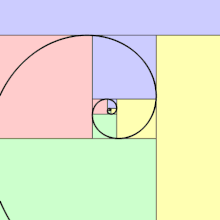
\includegraphics[scale=0.45]{Magazines/img/Vol1/fibonacci_seq.png}
\end{center}

Mr. Ballard himself also had some comments on the puzzle. He finds it interesting “because there are surprises in it; you start with the simple rules of a game, and you realize that you’ve discovered another way of generating the Fibonacci numbers”—which turn out to be hidden in the set of winning stone-piles for Bill (the second player). In addition, Mr. Ballard notes that, “just from looking at the puzzle, you would never see the Fibonacci numbers or the golden ratio.”

\epigraph{The connections between things…these connections are delightful discoveries in math.}{Mr. Dean Ballard}

Many math puzzles are like this – countless trials of seemingly random games, endless rows of numbers marching down the page. From the fractal symmetry of snowflakes to the golden-ratio spirals of mollusks to the geometric structure of the buckminsterfullerene molecule, nature hints us with simple yet intricate patterns, guiding us towards elegant perfection. After a long period of head-scratching, wall-punching, or muttered obscenities, you might at last find the answer.


So, go play the game with friends or family. You might get to solve one of the mysteries in your life, and who knows: you might even get to (re)visit sixth-grade math again.

\begin{center}
    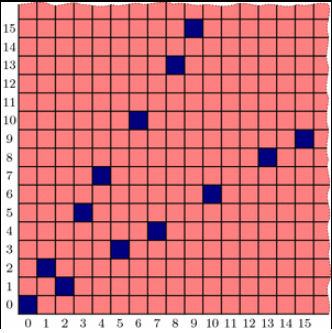
\includegraphics[scale=0.8]{Magazines/img/Vol1/wythoff_game.png}
\end{center}

Comment: if you’re curious to learn more about the game, it’s called Wythoff’s Game of Nim. First studied by W. A. Wythoff in 1907, it gained popularity after being featured in Martin Gardner’s famous Scientific American column, “Mathematical Games.”
\closearticle

\articletitle{Po-Shen Loh: the Traveling Salesman of Mathematics}{Owen Xuan}{}

He runs down the hall, talking to himself, but nobody is surprised. Suddenly, he stops. Turns left. An office. His office at Carnegie Mellon University.

Born in Madison, Wisconsin to a family rich with math ideas, now-professor Po-Shen Loh has influenced thousands of young mathematicians in the interesting path of his life. If you took a student from the math forums of Art of Problem Solving (AoPS), nine out of ten times they would recognize his name.  Yet throughout his journey, Loh is humble and remains willing and eager to, in his words, “get his hands dirty and build something.”

Along with many others, I was witness to this “build something” aspect of Loh’s personality. We participated in his daily virtual “Ask Math Anything” streams, which often lasted over an hour, was there at his in-person talk in Seattle, and read with wonder about NOVID- a practical program created with abstract math that goes beyond COVID contact tracing.

“Ask Math Anything” streams were a lighthouse for that era for me. Streams were unorganized, in that the content wasn’t planned, but was reassuring because of their consistency and atmosphere. Viewers formed connections with other strangers from the shared experience of watching someone who truly had a passion for raising the interest of math and changing the way it was learned. (And from insisting that he wore a green shirt!) As each stream started, these viewers would ask their questions, sometimes hitting the core of what it meant to learn math, other times presenting a math problem they found intriguing. Loh would answer these questions, demonstrating a profound capability to dissolve hard problems in easy concepts. April brought the end of the streams. In one of the final AMAs, Loh shared his newest project (viewers knew about it before the U.S. government!): NOVID.
\begin{center}
    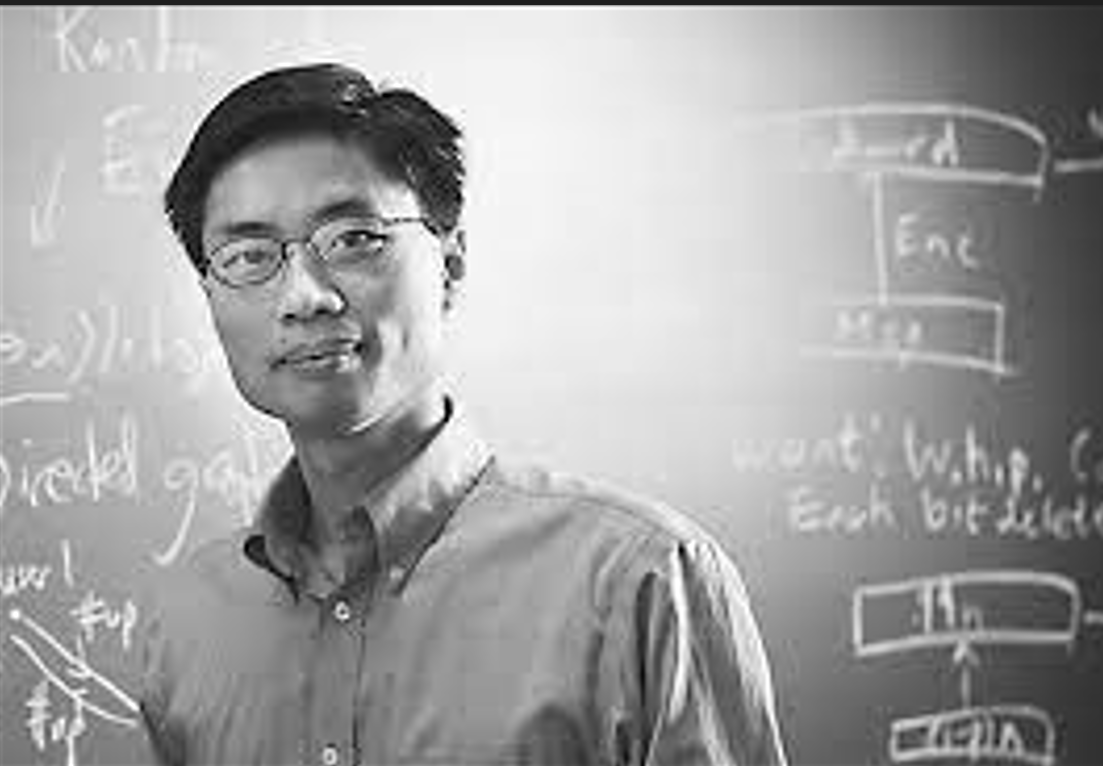
\includegraphics[scale=0.35]{Magazines/img/Vol1/po-shen loh.png}
\end{center}

“If you see some task that you’ve never seen before, can you actually invent a new approach to it?” By this quote, we see not only Loh’s focus on inventing-based learning, but a reflection of his values in his work. In a 21-page paper, Loh said the app will “introduce a fundamentally different paradigm for contact tracing”---it’s innovation in the best sense. In essence, Loh had created a type of “6 degrees of Kevin Bacon” for tracking the coronavirus; instead of only alerting a person after exposure, the app used various sensors to notify each person (before exposure) of how many relationship ‘degrees’ an infectious person has from them. If a friend of a friend contracted the virus, that would be two degrees of separation. This type of thinking falls under the umbrella term “network theory”, which was a basis of the envisioning of NOVID in prototype. Now, the app has reached over 100,000 users.

Four months after the streams ended, Loh gave a talk at Seattle, on a stage overlooking a grassy hill. Before the event started, Loh set up the entire stage, microphone, and speakers- with no crew. Later, I would learn that these trips marked the rebooting of his nation-wide tour before the pandemic. As we listened, the “traveling salesman of mathematics,” as Loh refers to himself, described how his combinatorial background applied to games, parties, Ramsey theory and NOVID. He tells us his goal is “to build the world to be a more thinking place.” Later, as it started to drizzle and Loh began to pack up, a few others and I approached Loh to ask questions and talk. He was friendly and willing to answer questions, and left Washington slightly soaked and having inspired dozens. Everything was perfect! Until he tested COVID-positive, with me as his last contact. (I swear it wasn’t me.)

The man running down the hall is Po-Shen Loh. He hurries to try to “milk every second”. Chances are, in that second, he’s thinking about making the world a more thinking place.
\closearticle

\articletitle{2022 Summer Reading Challenge: Infinite Powers}{Samarth Das}{}

The title of the book is called “Infinite Powers.” This gives an idea of a superhero story. The
story is about the mathematical superhero. Calculus is the branch of mathematics that gives you
infinite powers; most technology nowadays is based on these simplistic ideas. It also showcases
the hardwork of many people before us; the many scientists who had the guts and wits to
pioneer an idea that at the time was considered completely absurd. It is the work of these
unique people who we rely on till date for our technology. The journey from infinity to the modern
world is one that has been ignored at large and finally is exemplified in this book.

\begin{center}
   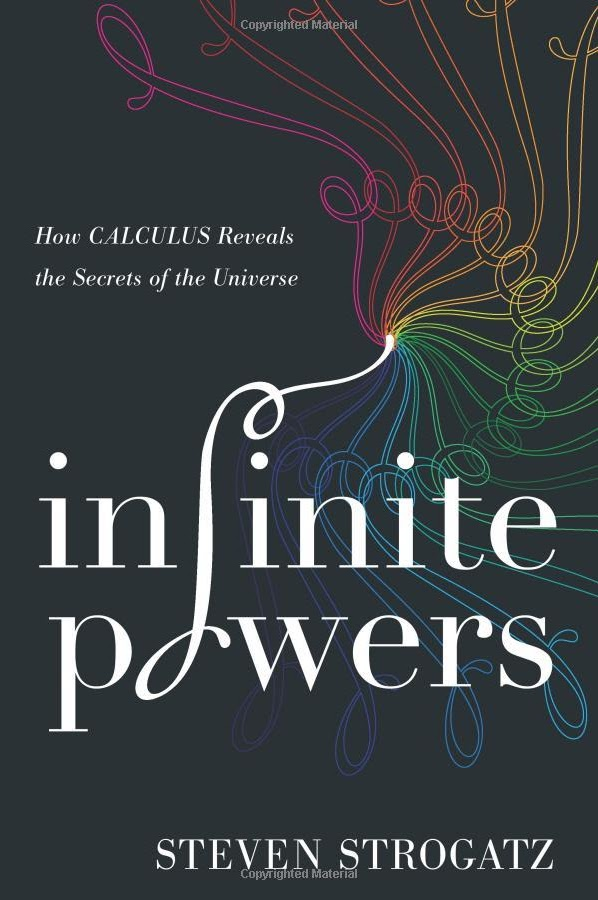
\includegraphics[scale=0.25]{Magazines/img/Vol1/infinity_powers.jpg}
\end{center}

The story starts off with the notion of infinity. It shows that infinity has created many issues in
ancient society, from executions to a disregarding of an entire field of mathematics. Many
ancient philosophers believed that it was something dangerous and broke all laws of
mathematics at the time. Philosophers like Zeno came up with “paradoxes” that showed how
infinity was an untamed animal. This remained for about two hundred years until Archimedes
came along. He knew how to harness infinity and work with it.
Archimedes was a pioneer of calculus because he came up with the ideas of cutting
unmeasurable objects into smaller measurable objects, an integral. He also came up with the
ideas of limits, which were essential for calculus because they proved that not all seemingly
infinite things are actually infinite. Thus concludes the ancient era of mathematics, since there
were no new developments for over eighteen hundred years.
People such as Galilieo, Descartes, and Newton came along and the mathematical
advancements rapidly developed. It started with the laws of planetary motion by Kepler. Then
Descartes arrived at the scene with the coordinate plane, a combination of algebra and
geometry. This was used by Newton to devise the laws of motion. With this came the great
acceleration of mathematics during the Scientific Revolution. Calculus was official now with
Leibiniz and Newton’s work, and it started to spill into other fields.
Calculus became quickly essential in the engineering field. Construction of automatons and
other machines such as trains were made much more efficient. It was an important part of the
First Industrial Revolution. Then came World War I and II, where the technological
advancements were heavily used. The atomic bomb would not have been possible without
calculus insight, and so would much of our military equipment today ranging from satellite
systems to tanks. Following this came the Cold War. Advancements such as in the Space Race
would not have been possible without calculus. We would have never landed on the moon. As
of today, it has extended into almost all fields of science, from medicine to space.
The idea of pure mathematics being applied to other disciplines appealed to me. I recalled an
experience I had earlier regarding mathematics. As I learned calculus, I was able to apply it to
my physics studies and beyond. I realized that there is a whole new world out here; that there
are many fields of research that have stemmed from one basic idea. A story about mathematics
history transforms oneself into an omniscient.
\closearticle

\articletitle{2022 Summer Reading Challenge: Fermat’s Enigma}{Jason yao}{}

A while ago, I was reading “Fermat’s Enigma”, by Simon Singh. Although two and a half decades old, I was still struck by the story behind the century-old problem. The book offered a glimpse into the concept of mathematical proof. A complete proof, much like mathematics as a whole, is like a house of cards, where the entire structure breaks down if one part does. Unlike the case in science, evidence is not enough. “Fermat’s enigma” details the four-hundred-year story behind Fermat’s last theorem, a small riddle posed by Fermat, who was known as the “prince of amateurs” among mathematicians. Although undoubtedly a great story, it was the concept of mathematical proof inside that interested me the most.

Proofs are generally agreed to have been used as early as ancient Greek times, and is acknowledged as one of the greatest achievements of Greek mathematicians, notably Euclid. Although they were mostly limited to geometry, he still revolutionized proofs in general. His book, “The Elements” lays the foundation for this, and as such is often regarded as the mathematical bible. Nowadays, proof theory treats proofs as inductively defined steps, and sometimes does not even require an assumption that axioms are true. This allows parallel theories as models of a concept to be considered, based on different sets of axioms. For example, non-Euclidean structures. However, the majority of mathematics is done with the general set of postulates.

 
A mathematical proof should be seamless from start to finish in order to be accepted. They are heavily dependent on previous theorems, and if a theorem is just slightly incorrect, every theorem that relies on it will also end up being unacceptable. Even evidence that a theorem works for every single number until the trillions, it is not proof that the theorem must be true.
\begin{center}
   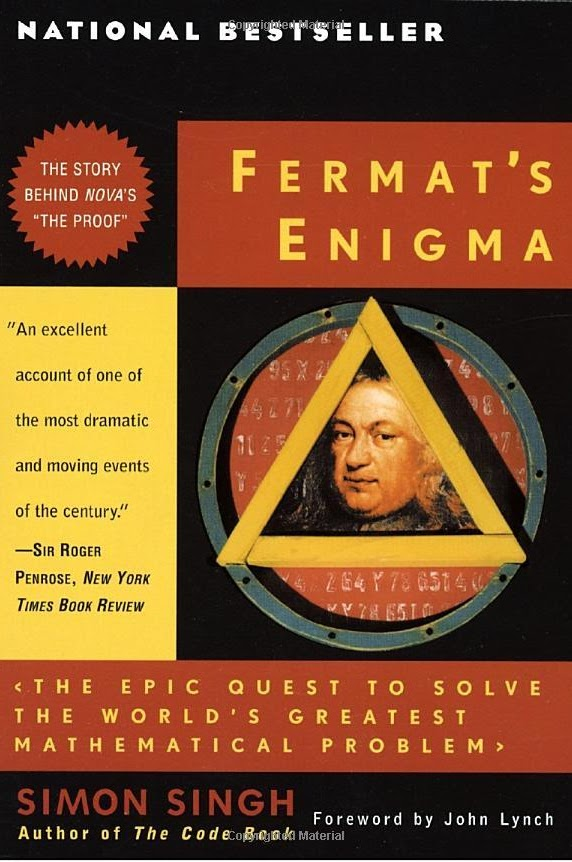
\includegraphics[scale=0.25]{Magazines/img/Vol1/fermats_enigma.jpg}
\end{center}
For example, a hypothesis by Leonard Euler, his Leonard of Powers Conjecture, is true for every number until 61917364224 (about 61 trillion). It could be worse however, for example, $n^{17}+9$ and $(n+1)^{17} + 9$ are relatively prime until $842443292559288932928819732230890$
$0672459420460792433$. There is no reason further conjectures are not as deceptive as either one of these. 

Mathematics is like the construction of an ever-growing structure made out of plywood. If one part rots or breaks, everything on top of it does too. Therefore, an acceptable proof is made out of irrefutable, logical, mathematical steps, which lead to a conclusion. The cornerstones are postulates, axioms, and definitions, things that are assumed to be true, and what things mean. For example, an example of a postulate is that for numbers $a$ and $b$, $a + b = b + a$. From these postulates, theorems, laws, and identities can be constructed, which can be used to construct more theorems, laws, and identities. A statement that is thought to be true but not proven so is known as a conjecture, or a hypothesis if frequently used as an assumption to create further progress if true. On a tangential sidenote, certain statements can be proven to be undecidable, which means that based on the accepted axioms, they cannot be proven to be true or false. 

Overall, a proof has a sacred meaning, it is the holy grail of math. Only a complete line of reasoning can be used in mainstream mathematics, because only they are acceptable. It is a rigorous and sometimes tedious process, but a necessary and almost romantic concept.
\end{multicols}
\closearticle

% End of magazine
\begin{multicols}{2}
  \begin{center}
      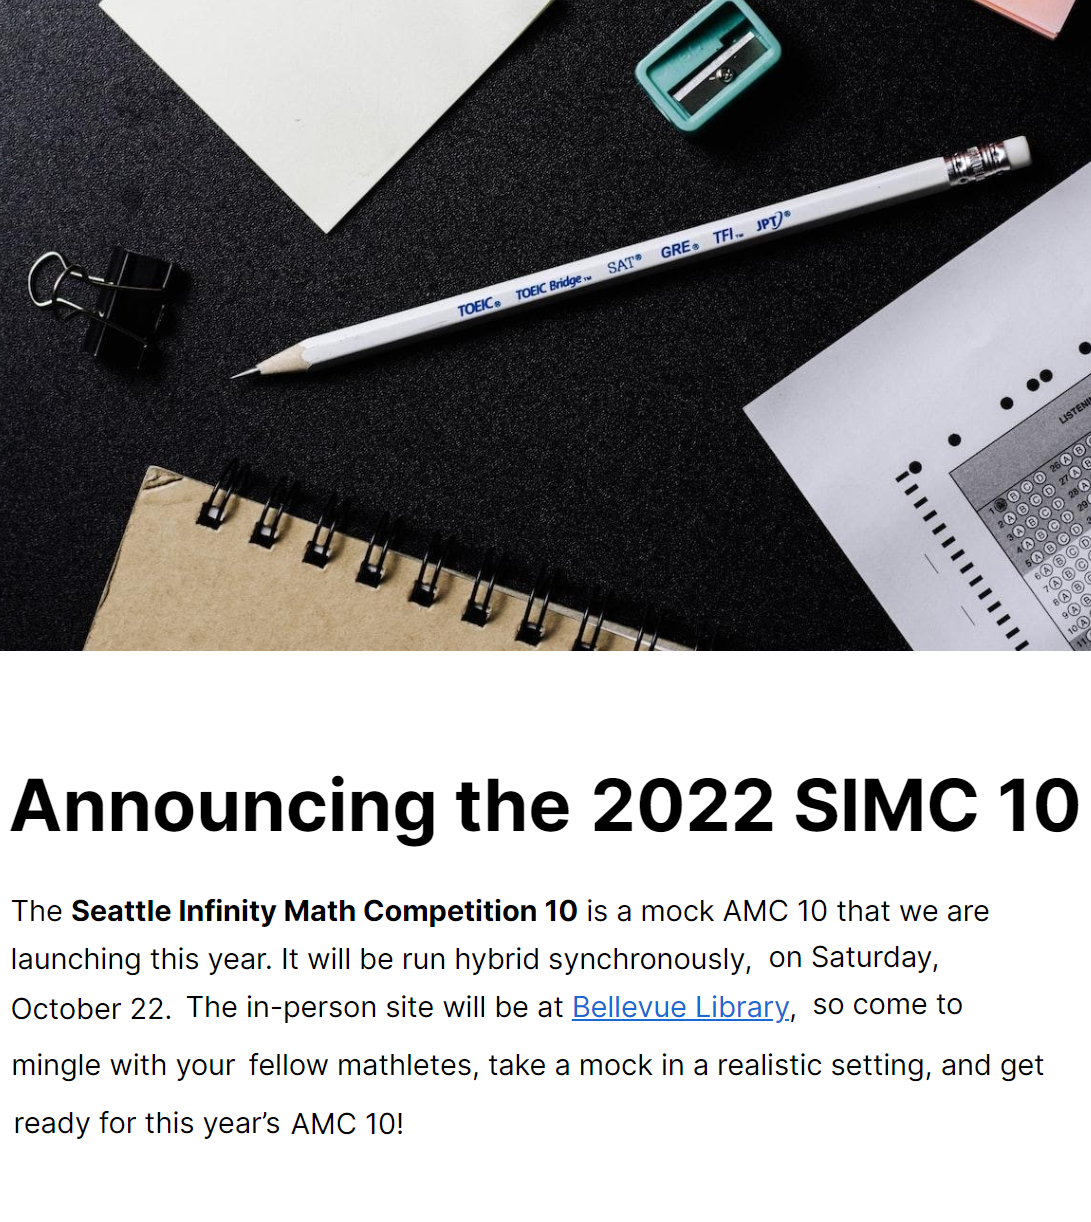
\includegraphics[scale=0.25]{Magazines/img/Vol1/simc10.png}
  \end{center}

\clearcolumn
\;

{\hspace{24mm} \sc\Large{\textbf{Contact Us}}}
\vspace{0.5mm}
\begin{center}
\begin{tabular}{c l}
  
\includegraphics[scale=0.06,valign=c]{Magazines/img/email.png}
    & \href{mailto:seattleinfinitymathcircle@gmail.com}{Email}\\
  \;\\
  
\includegraphics[scale=0.1,valign=c]{Magazines/img/website.png}
    & \href{https://seattleinfinity.org}{Website} \\
  
\includegraphics[scale=0.5,valign=c]{Magazines/img/facebook.png}
    & \href{https://www.facebook.com/simathcircle/}{Facebook} \\
  
\includegraphics[scale=0.5,valign=c]{Magazines/img/insta.png}
    & \href{https://www.instagram.com/seattleinfinitymathcircle/}{Instagram} \\
  
\includegraphics[scale=0.5,valign=c]{Magazines/img/youtube.png}
    & \href{https://www.youtube.com/channel/UCgwA-iysWPc_XG0R0AZ5z5g/videos}{YouTube} \\
  
\includegraphics[scale=0.013,valign=c]{Magazines/img/discord.png}
    & \href{https://discord.gg/2Ma3dURhTt}{Discord} 
\end{tabular}
\end{center}    
\end{multicols}

\end{document}
